

\pgfplotsset{compat=1.14}
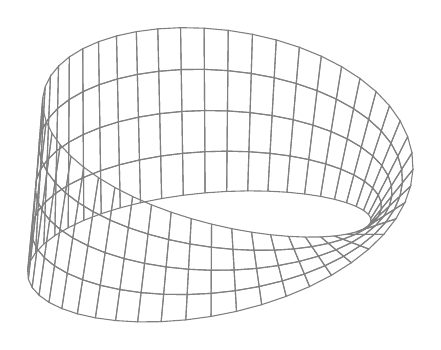
\begin{tikzpicture}
  \begin{axis}
    [
      hide axis,
      view={40}{40}
    ]
    \addplot3
    [
      surf,
      mesh, 
      shader=faceted interp,
      point meta=x,
      draw=gray,
      %colormap/blackwhite,
      samples=50,
      samples y=5,
      z buffer=sort,
      domain=0:360,
      y domain=-0.25:0.25,
    ]
    (%
      {(1+0.5*y*cos(x/2)))*cos(x)},
      {(1+0.5*y*cos(x/2)))*sin(x)},
      {0.5*y*sin(x/2)}
    );
    
%    % This is supposed to draw surface normals (I guess) - but it seems to be wrong:
%    \addplot3
%    [
%      samples=90,
%      %domain=-145:180,
%      domain=0:360,
%      samples y=0,
%      thick,
%      postaction={decorate},
%      decoration={% pgfplots manual 355-356
%        markings,
%        mark=between positions 0 and 1 step 10mm with
%        {
%          \node [single arrow, transform shape, rotate=-90, fill, draw, inner sep=0pt, single arrow head extend=1pt, text width=2.5mm, text height=0pt, anchor=west, line width=.4pt, ] {};
%        },
%      },
%    ]
%    (%
%      {cos(x)},
%      {sin(x)},
%      {0}%
%    );
    
    
  \end{axis}
\end{tikzpicture}


% See also:
% https://tex.stackexchange.com/questions/496801/moebius-strip-border
% this draws a border - which is also interesting. We want a border *and* surface normals!


% Yet another variant:
% https://tex.stackexchange.com/questions/364073/adding-lines-perpendicular-in-the-plane-to-a-mobius-band
%\begin{tikzpicture}
%\begin{axis}[
%hide axis,
%view={40}{40}
%]
%\addplot3 [
%mesh, shader=faceted interp,
%point meta=x,
%colormap/blackwhite,
%samples=100,
%samples y=5,
%z buffer=sort,
%domain=0:360,
%y domain=-0.5:0.5
%] (
%{(1+0.5*y*cos(x/2)))*cos(x)},
%{(1+0.5*y*cos(x/2)))*sin(x)},
%{0.5*y*sin(x/2)});
%
%\addplot3 [
%samples=50,
%domain=-145:180,
%samples y=0,
%thick
%] (
%{cos(x)},
%{sin(x)},
%{0});
%\end{axis}
%\end{tikzpicture}